\documentclass[11pt]{article}
\usepackage{amsmath,textcomp,amssymb,graphicx,comment,tikz}
\usepackage[margin=0.75in]{geometry}
\usetikzlibrary{arrows}
\newcommand{\tab}{\hspace*{2em}}

\def\NameA{Alvin Wong, cs189-cq, 22655478}  % Your name
\def\NameB{Chun Yin Yau, cs189-em, 24023460}

\title{CS189--Spring 2014 --- Solutions to Homework 1}
\author{\NameA || \NameB}
\markboth{CS199--Sp 2014 HW1 \NameA , \NameB }{CS189--Sp 2014 HW1 \NameA,  \NameB}
\pagestyle{myheadings}

\begin{document}
\maketitle

\section*{1.} 
\textbf{Question:} Train a linear SVM using raw pixels as features. Plot the error rate on the test set versus the number of training examples. State your choice of parameters for training the SVM.
\\\\
Our code for this problem can be executed by calling q1() inside the code subdirectory.
\\\\
Brief Description of what we did: Our code loads all the 7 sets of training data, then configures the feature matrix in a m x 784 matrix. m is the number of training examples for each of the 7 sets. This gets passed as input to train, where the SVM algorithm gives us a model with the best fit parameters. We use this model to predict on our test set, and output the error rates as a function of the size of the training data.
\\\\
Plot: (X-axis: size of training set, Y-axis: error rate on test set.)
\begin{figure}[ht!]
\centering
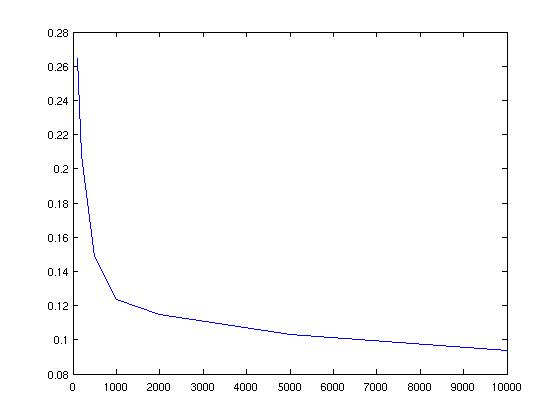
\includegraphics[width=100mm]{figq1.jpg}
\caption{Plot comparing the error rate on the test set with different sized training sets.}
\label{overflow}
\end{figure}
\\
Analysis: This makes sense -- more data improves the accuracy of the classifier.
\\\\
Parameters for the SVM: We played around with the C values and found an improvement on using small C's. The C value we used as a parameter was 0.0000002. (chosen by fidgeting with values) We also provided the -q flag to mute output in the SVM. This gives us an accuracy of 90.6 percent (error rate of 9.4 percent) on the test set using the 10k training set.
\newpage

\section*{2.}
\textbf{Question:} Create confusion matrices for your experiments in Problem 1. Color code your results and report them. What insights can you get about the performance of your algorithm from looking at the confusion matrix?
\\\\
Our code for this problem can be executed by calling q2() inside the code subdirectory. According to a Piazza post (@15), we only need to include the confusion matrix for the 10k training set. Below is the plot. Plot: (Note: labels are incorrect., shift them by 1 less [not sure how to do that in matlab]). X-axis: Actual class label (needs to be shifted by 1), Y-axis: Predicted class label (needs to be shifted by 1).
\begin{figure}[ht!]
\centering
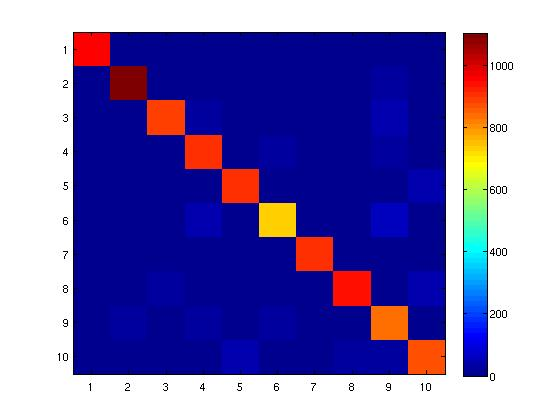
\includegraphics[width=100mm]{figq2.jpg}
\caption{Confusion Matrix for the Test Set using the Model Trained on the 10k Training Set.}
\label{overflow}
\end{figure}
\\
\begin{table}[ht]
\caption{Confusion Matrix}
\centering
\begin{tabular}{c | c c c c c c c c c c }
\hline\hline
X & 0 & 1 & 2 & 3 & 4 & 5 & 6 & 7 & 8 & 9 \\
\hline
0 & 958 & 0 & 1 & 1 & 0 & 3 & 9 & 2 & 5 & 1 \\
1 & 0 & 1106 & 2 & 3 & 1 & 0 & 4 & 1 & 18 & 0 \\
2 & 8 & 7 & 898 & 23 & 10 & 1 & 16 & 15 & 48 & 6 \\
3 & 6 & 1 & 16 & 909 & 2 & 24 & 3 & 12 & 24 & 13 \\
4 & 1 & 0 & 7 & 1 & 903 & 0 & 10 & 1 & 13 & 46 \\
5 & 11 & 5 & 5 & 37 & 14 & 732 & 17 & 9 & 53 & 9 \\
6 & 10 & 3 & 5 & 1 & 8 & 14 & 909 & 0 & 8 & 0 \\
7 & 0 & 12 & 22 & 3 & 9 & 1 & 1 & 937 & 5 & 38 \\
8 & 11 & 19 & 8 & 25 & 10 & 31 & 10 & 15 & 830 & 15 \\
9 & 11 & 6 & 2 & 15 & 47 & 4 & 0 & 27 & 19 & 878 \\
\end{tabular}
\end{table}
\\\\
Above Matrix: The horizontal 0-9 refers to the predicted labels. The vertical 0-9 refers to the actual labels.
\\\\
Analysis: The confusion matrix provides us a lot of insight to analyzing our classifier. For example, we can get the accuracy on the classifier on our test set by taking the sum of entries along the diagonal of the matrix and dividing by the total number of labels. Further, we can see which types of digits we are more likely to misclassify. for example, in the diagram,notice that there's a light blue area in the coordinates (9,6). This corresponds to classifying images that are actually "8", with the label "5". It logically makes sense, they look similar. We can go the other way around. "4" and "9" are pretty similar, so let's look at the coordinates (10,5). Indeed, the blue area is a bit more lighter, meaning on the scale, there are more misclassifications between predicting "4" when the image is actually "9". You can even further compute probabilities of predicting a value given the actual label. For example, the probability we predict "5" when the actual label is "1" is the value corresponding to these labels [ (6,2) on the graph ], divided by the sum of entries in the row labeled 2 in the diagram (corresponding to label '1').
\\\\

\section*{3.}
\textbf{Question:} Explain why cross-validation helps. Find the optimal value of the parameter 'C' using 10-fold cross-validation on the training set with 10,000 examples. Train an SVM with this value of 'C' and report the test error rate.
\\\\
Why Cross-Validation? In 10-fold cross-validation on the 10k training set, first, we pick a value for the parameter 'C'. We need to repeat a training procedure 10 times. We first divide the training set into 10 chunks of 1k data. We train on 9 of these 1k folds, and use the other 1k fold to evaluate our accuracy on the classifier using the parameters learned from training on the 9k set. We repeat this for each of the 1k folds, which means that we train 10 times, and each time, we have an error rate associated against the validation set. We average these accuracies to get a mean accuracy, which should accurately reflect the accuracy on the test set. Note that we haven't exposed our model to the test data yet, we've gotten a somewhat accurate measurement for this particular 'C' value that we chose. In practice, we would probably run k-fold cross-validation multiple times on a particular value of 'C' to get a more accurate measurement, since randomness does play a role in how the data gets separated.
\\\\
Now, how do we know that this current 'C' is good? Well, we don't yet, so we repeat this procedure for different 'C' values. By analyzing the mean error rate on the validation set, we effectively compute a reasonable estimate for the actual test error. Once we searched some 'C' values and fine tuned a good estimate for 'C', now we can train on the entire training set with this optimal 'C' value, and then evaluate the accuracy on the test set. This is the power of cross-validation -- fine tuning your hyperparameters, which has an effect of influencing the choice of parameters for our classifier.
\\\\
You can run our code, which has two implementations. The 10-fold cross-validation process is the same; however, the choices of which 'C' to consider are different. You can run q3a() to make our classifier train on the 10k set, with 10-fold cross-validation, on C values being powers of ten from -10 to 0. We also seeded the RNG so that the results reported here should be the same as you run it. When we run our code, we get an optimal C value of $1e-7$, with an error rate on the test set of 9.53 percent.
\\\\
We have a slightly more elaborate search algorithm that makes use of the information run in q3a. You can run q3b() to test this out. We consider possible C ranges in $[10^{-7.5}, 10^{-6.5}]$, and we partition the range of exponents $[-7.5,-6.5]$ into 8 equidistant numbers. We compute 10-fold cross-validation with these 6 C values, and then we pick the best C so far. We narrow down the range of exponents centered at the bestC value, and run this 8-point algorithm again twice (to save time). Ideally would we run the k-fold procedure more times on the same C value to get a better accuracy due to potential randomness. When we run our code (which is a bit longer), we get an optimal C value of $2.7465e-07$, with an error rate on the test set of 9.41 percent.

\end{document}
